%%%%%%%%%%%%%%%%%%%%%%%%%%%%%%%%%%%%%%%%%%%%%%%%%%%%%%%%%%%%%%%%%%%%%%%%%%%%%%%%
% Modelo para documentação de LABS, PSETS, etc.
%
% Por: Abrantes Araújo Silva Filho
%      abrantesasf@gmail.com


%%%%%%%%%%%%%%%%%%%%%%%%%%%%%%%%%%%%%%%%%%%%%%%%%%%%%%%%%%%%%%%%%%%%%%%%%%%%%%%%
%%% Classe do documento
\documentclass[12pt]{article}

%%%%%%%%%%%%%%%%%%%%%%%%%%%%%%%%%%%%%%%%%%%%%%%%%%%%%%%%%%%%%%%%%%%%%%%%%%%%%%%%
%%% Preâmbulo com todas as outras outras chamadas para todos os outros packages
%%% e o que mais for necessário
\input{utils/preambulo.tex}

%%%%%%%%%%%%%%%%%%%%%%%%%%%%%%%%%%%%%%%%%%%%%%%%%%%%%%%%%%%%%%%%%%%%%%%%%%%%%%%%
%%% Ajuste do layout, espaçamento de linhas e etc.:
\geometry{a4paper, portrait, twoside, %left=1.5in, hmarginratio=2:3,
bindingoffset=0in}
%\onehalfspacing

%%%%%%%%%%%%%%%%%%%%%%%%%%%%%%%%%%%%%%%%%%%%%%%%%%%%%%%%%%%%%%%%%%%%%%%%%%%%%%%%
%%% Configurações para as propriedades do PDF:
\hypersetup{
   hidelinks,           % Comente para web, descomente para impressão
   colorlinks=true,    % True para web, False para impressão
   pdftitle={Uso do papel almaço},
   pdfauthor={Abrantes Araújo Silva Filho},
   pdfsubject={Escrita de trabalhos acadêmicos},
   pdfkeywords={almaço, manuscrito},
   pdfinfo={
      CreationDate={}, % Ex.: D:AAAAMMDDHH24MISS
      ModDate={}       % Ex.: D:AAAAMMDDHH24MISS
   }
}

%%%%%%%%%%%%%%%%%%%%%%%%%%%%%%%%%%%%%%%%%%%%%%%%%%%%%%%%%%%%%%%%%%%%%%%%%%%%%%%%
%%% Compilação condicional de capítulos
%\includeonly{}

%%%%%%%%%%%%%%%%%%%%%%%%%%%%%%%%%%%%%%%%%%%%%%%%%%%%%%%%%%%%%%%%%%%%%%%%%%%%%%%%
%%% Começa o documento
\begin{document}

%%%%%%%%%%%%%%%%%%%%%%%%%%%%%%%%%%%%%%%%%%%%%%%%%%%%%%%%%%%%%%%%%%%%%%%%%%%%%%%%
%%% Front matter
\pdfbookmark[1]{Uso do papel almaço}{titulo}
\title{\textbf{Uso do papel almaço}}
\author{Abrantes Araújo Silva Filho}
\date{2023-05-31}
\maketitle
\renewcommand{\abstractname}{\textbf{Resumo}}
\abstract{\noindent Aprenda a usar corretamente o papal almaço para fazer seus
trabalhos acadêmicos de forma manuscrita. Muitos alunos começam o ensino
superior sem nunca ter utilizado papel almaço em seus trabalhos acadêmicos e,
por incrível que pareça, quando solicitados a entregar um trabalho manuscrito
com esse tipo de papel, cometem erros básicos como escrever com o papel de
cabeça para baixo, escrever de trás para frente, cortar as folhas, rasurar e
amassar o papel. Este pequeno texto é um ``guia de uso'' do papel almaço.}
%\pdfbookmark[1]{Sumário}{sumario}
%\tableofcontents

%%%%%%%%%%%%%%%%%%%%%%%%%%%%%%%%%%%%%%%%%%%%%%%%%%%%%%%%%%%%%%%%%%%%%%%%%%%%%%%%
%%% Main matter
%\newpage
%%%%%%%%%%%%%%%%%%%%%%%%%%%%%%%%%%%%%%%%%%%%%%%%%%%%%%%%%%%%%%%%%%%%%%%%%%%%%%%%
\section{O papel almaço}
\label{sec:intro}

O \textbf{papel almaço} tem esse nome devido a uma antiga expressão portuguesa,
``à lo maço'', que se referia à venda desse papel em blocos com grandes
quantidades \cite{almaco2017}.

O papel almaço é um tipo de papel que equivale, aproximadamente, a duas folhas
de caderno, unidas (sem espiral ou encadernação). O papel almaço é encontrado em
diversos formatos e características, por exemplo:

\begin{itemize}
\item Pauta: pode ser pautado, não pautado ou quadriculado;
\item Margem: pode ter uma ou mais margens, do lado direito e/ou esquerdo de
      cada folha;
\item Formato: A4, ofício ou outros; e
\item Cor: branca, creme e outras.
\end{itemize}

É um papel muito utilizado para trabalhos acadêmicos manuscritos, provas e
rascunhos diversos. A figura~\ref{fig:papel}, a seguir, ilustra alguns tipos
de papel almaço comumente encontrados no mercado.

\begin{figure}[H]
\centering
\caption{Tipos de papel almaço}
\label{fig:papel}
\vspace{-0.3cm}
%\fbox{

\includegraphics[scale=0.3]{imagens/tipos.png}
%}\\
%\footnotesize{Fonte: xxx}
\end{figure}

Este texto é um pequeno guia de como usar corretamente o papel almaço em seus
trabalhos acadêmicos.


%%%%%%%%%%%%%%%%%%%%%%%%%%%%%%%%%%%%%%%%%%%%%%%%%%%%%%%%%%%%%%%%%%%%%%%%%%%%%%%%
\section{Como usar o papel almaço?}
\label{sec:como}


%%%%%%%%%%%%%%%%%%%%%%%%%%%%%%%%%%%%%%%%%
\subsection{Orientação}
\label{sec:como-orientacao}

O papel almaço deve ser utilizado com o lado de união das folhas à esquerda, e
com o cabeçalho na parte de cima, como na figura~\ref{fig:orientacao}.

\begin{figure}[H]
\centering
\caption{Orientação correta do papel almaço}
\label{fig:orientacao}
\vspace{-0.3cm}
%\fbox{

\includegraphics[scale=0.35]{imagens/almaco3.png}
%}\\
%\footnotesize{Fonte: xxx}
\end{figure}

Muitos alunos começam a escrever com o papel almaço de cabeça para baixo, com o
lado de união das folhas à direita e, por vezes, de trás para frente. A
figura~\ref{fig:orienterrado} ilustra alguns erros na orientação do papel.

\begin{figure}[H]
\centering
\caption{Orientações incorretas do papel almaço}
\label{fig:orienterrado}
\vspace{-0.3cm}
%\fbox{
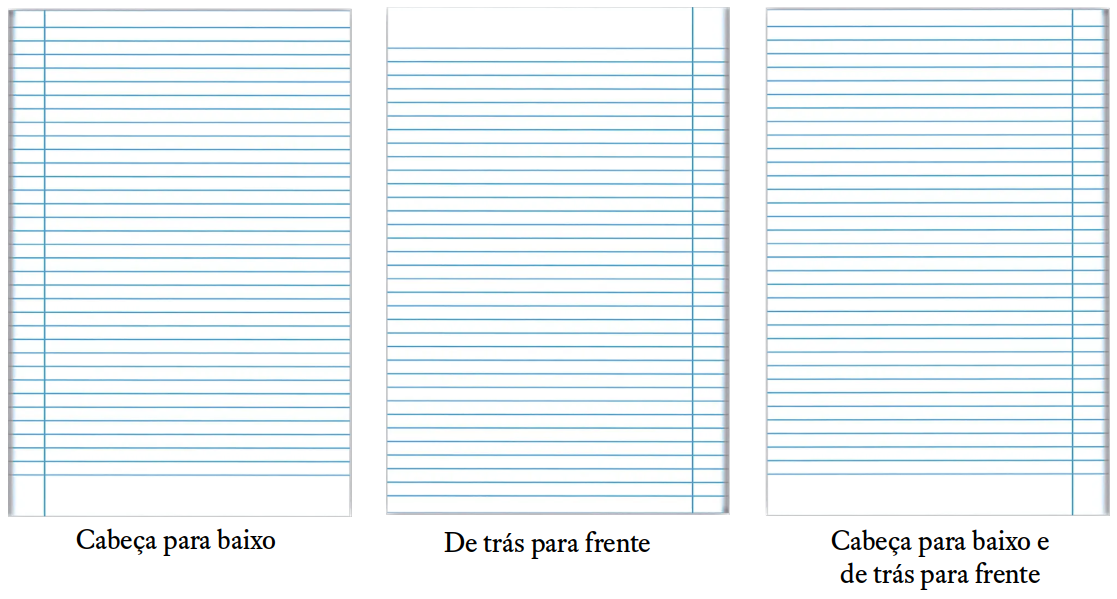
\includegraphics[scale=0.3]{imagens/orienterrado.png}
%}\\
%\footnotesize{Fonte: xxx}
\end{figure}


%%%%%%%%%%%%%%%%%%%%%%%%%%%%%%%%%%%%%%%%%
\subsection{Tamanho, cor, pauta}
\label{sec:como-a4}

Cada professor tem preferência por um tipo específico de papel almaço. Siga
\textbf{exatamente} o modelo que seu professor indicar, em termos de tamanho,
cor e tipo de pauta! Os professores não são obrigados a aceitar trabalhos com
papel fora do especificado.

Tome cuidado pois algumas papelarias vendem papel almaço no formato A4 que não
são exatamente na medida do papel A4 (\qty{297}{\milli\meter} $\times$
\qty{210}{\milli\meter}). Uma variação pequena, de alguns milímetros, é
aceitável. Mas não entregue uma papel de tamanho ofício ou carta se o professor
especificou um papel no formato A4.

Cuidado com o tipo de pauta: se o professor especificou papel almaço pautado,
não utilize outros tipos como papel almaço quadriculado.


%%%%%%%%%%%%%%%%%%%%%%%%%%%%%%%%%%%%%%%%%
\subsection{Margem}
\label{sec:como-margem}

Se o papel almaço que você está utilizando não possuir a linha de marcação da
margem, faça uma dobradura leve no papel onde estaria a linha de margem. Desse
modo todas as páginas estarão com a margem marcada.



%%%%%%%%%%%%%%%%%%%%%%%%%%%%%%%%%%%%%%%%%
\subsection{Lápis ou caneta?}
\label{sec:como-lapis}

Siga as instruções de seu professor. Alguns trabalhos deve ser escritos à
caneta, outros à lápis.

Se utilizar lápis, dê preferência para modelos com grafite escuro (2B, 4B ou
6B). Não utilize lápis de cor clara (HB). Se utilizar caneta, tenha certeza de
não rasurar o papel.


%%%%%%%%%%%%%%%%%%%%%%%%%%%%%%%%%%%%%%%%%
\subsection{Corte do papel}
\label{sec:como-corte}

Nunca, em hipótese nenhuma, corte o papel almaço no meio. Nunca entregue apenas
meia folha de almaço.


%%%%%%%%%%%%%%%%%%%%%%%%%%%%%%%%%%%%%%%%%
\subsection{Letra cursiva ou de forma?}
\label{sec:como-cursiva}

Todos os trabalhos manuscritos em papel almaço devem ser escritos com
\textbf{letra cursiva}. Não utilize letra de forma maiúscula, você deve
demonstrar que sabe distinguir o uso de letras maiúsculas e minúsculas. Além
disso lembre-se de que a letra deve \textbf{ser legível}.



%%%%%%%%%%%%%%%%%%%%%%%%%%%%%%%%%%%%%%%%%
\subsection{Cabeçalho}
\label{sec:como-cabecalho}

Comece a escrever na primeira linha, com o \textbf{cabeçalho} de
identificação. Se o professor indicar um modelo específico de cabeçalho, siga as
instruções do professor. Se o professor não indicar um modelo específico de
cabeçalho, escreva o nome da instituição, o curso, o nome completo do professor,
seu nome completo, sua turma e alguma informação de identificação, como seu
número de matrícula. A figura~\ref{fig:cabecalho} ilustra um bom cabeçalho.

\begin{figure}[H]
\centering
\caption{Modelo correto de cabeçalho}
\label{fig:cabecalho}
\vspace{-0.3cm}
%\fbox{
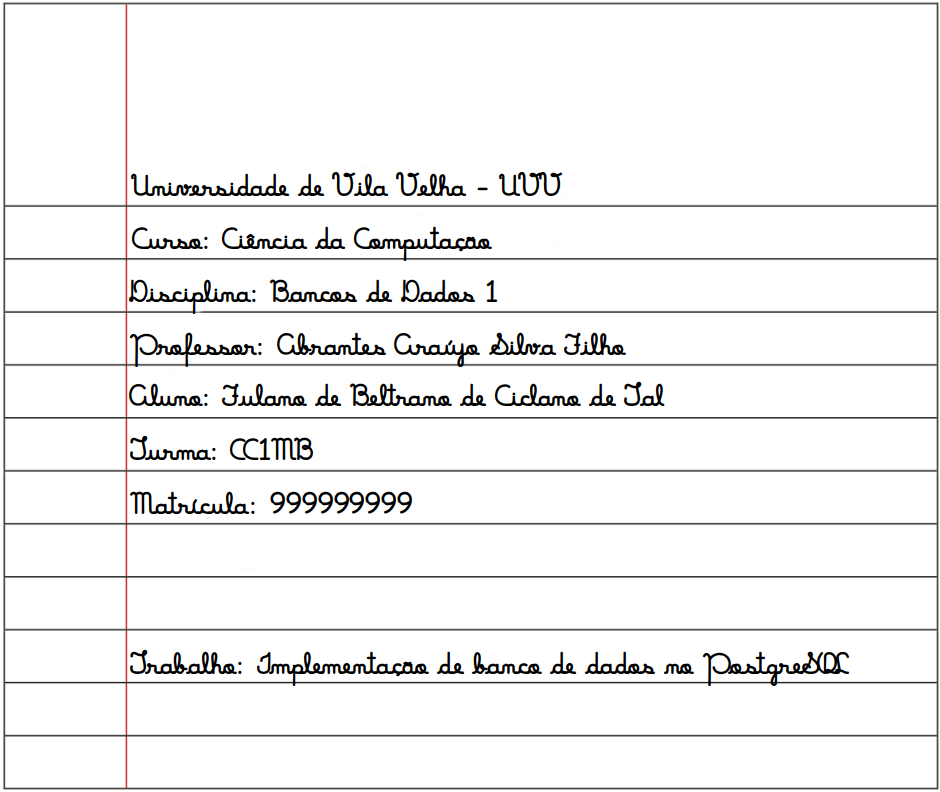
\includegraphics[scale=0.36]{imagens/cabecalho2.png}
%}\\
%\footnotesize{Fonte: xxx}
\end{figure}

Atenção: sempre coloque todos os nomes, inclusive os sobrenomes, por
extenso. Nunca abrevie os nomes pois podem existir alunos cujos nomes abreviados
são idênticos.


%%%%%%%%%%%%%%%%%%%%%%%%%%%%%%%%%%%%%%%%%
\subsection{Uso do verso}
\label{sec:como-verso}

Exceto se o seu professor explicitamente proibir, você deve utilizar normalmente
o verso das folhas do papel almaço. Isso diminui a quantidade de folhas a serem
utilizadas e organiza seu trabalho.

Quando utilizar o verso com lápis muito macio (4B, 6B ou outro), tenha cuidado
para não causar ``borrões'' nas páginas do anverso.



%%%%%%%%%%%%%%%%%%%%%%%%%%%%%%%%%%%%%%%%%
\subsection{Várias páginas e numeração}
\label{sec:como-varias}

Quando precisar utilizar mais de uma folha de papel almaço, não coloque umas
dentro das outras, como se fossem um caderno ou livro. Isso dificultará
enormemente a organização do texto.

Sempre que usar duas ou mais folhas de papel almaço, coloque-as umas após as
outras, numerando as folhas. A cada nova folha, \textbf{reescreva o
  cabeçalho}. Grampeie ou prenda as folhas com um clipe.
  
Se ocorrer sobra de um lado, nunca corte o papel almaço! Finalize seu trabalho e
entregue o papel almaço íntegro, sem cortes.


%%%%%%%%%%%%%%%%%%%%%%%%%%%%%%%%%%%%%%%%%
\subsection{Uso de capa}
\label{sec:como-capa}

Em geral não é necessário fazer uma capa para seu trabalho em papel almaço mas,
se deseja, pode colocá-lo em uma pasta fina para protegê-lo de sujeiras. A capa
também ajuda a evitar que o papel amasse sem querer.


%%%%%%%%%%%%%%%%%%%%%%%%%%%%%%%%%%%%%%%%%%%%%%%%%%%%%%%%%%%%%%%%%%%%%%%%%%%%%%%%
%%% Apêndices
%\newpage
%\appendix
%\input{apend/xxxx}

%%%%%%%%%%%%%%%%%%%%%%%%%%%%%%%%%%%%%%%%%%%%%%%%%%%%%%%%%%%%%%%%%%%%%%%%%%%%%%%%
%%% Back matter
\bibliography{utils/biblioteca}
%\printindex

%%%%%%%%%%%%%%%%%%%%%%%%%%%%%%%%%%%%%%%%%%%%%%%%%%%%%%%%%%%%%%%%%%%%%%%%%%%%%%%%
%%% Termina o documento
\end{document}
